\documentclass{article}
\usepackage{v-test-paper}
\title{\textsc{JEE Advanced 2022 Paper-II\\Physics}}
\newenvironment{solution}{\par\noindent\color{red!85!black}$\Rightarrow$\vspace{0em}}{}
\date{}
\begin{document}
\maketitle

\begin{enumerate}
    \item A particle of mass $1 \, \text{kg}$ is subjected to a force which depends on the position as $\vec{F} = -k(x\hat{i} + y\hat{j}) \, \text{kg m s}^{-2}$ with $k = 1 \, \text{kg s}^{-2}$. At time $t = 0$, the particle's position $\vec{r} = (1\hat{i} + \frac{1}{\sqrt{2}}\hat{j} + \frac{1}{2}\hat{k}) \, \text{m}$ and its velocity $\vec{v} = (-\frac{1}{\sqrt{2}}\hat{i} + \frac{1}{2}\hat{j} + 2\hat{k}) \, \text{m s}^{-1}$. Let $v_x$, and $v_y$ denote the $x$ and the $y$ components of the particle's velocity, respectively. Ignore gravity. When $z = 0.5 \, \text{m}$, the value of $(x_v - y_v)_{z}$ is \_\_\_ $\text{m}^2 \text{s}^{-1}$.
    
    \item In a radioactive decay chain reaction, $^{230}\text{Th}$ nucleus decays into $^{214}\text{Po}$ nucleus. The ratio of the number of $\alpha$ to number of $\beta^-$ particles emitted in this process is \_\_\_.
    
    \item Two resistances $R_1 = X \, \Omega$ and $R_2 = 1 \, \Omega$ are connected to a wire $AB$ of uniform resistivity, as shown in the figure. The radius of the wire varies linearly along its axis from $0.2 \, \text{mm}$ at $A$ to $1 \, \text{mm}$ at $B$. A galvanometer ($G$) connected to the center of the wire, $50 \, \text{cm}$ from each end along its axis, shows zero deflection when $A$ and $B$ are connected to a battery. The value of $X$ is \_\_\_.

    \begin{center}
        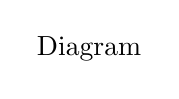
\begin{tikzpicture}
            \node {Diagram};
        \end{tikzpicture}
    \end{center}

    \item In a particular system of units, a physical quantity can be expressed in terms of the electric charge \( e \), electron mass \( m_e \), Planck's constant \( h \), and Coulomb's constant \( k = \frac{1}{4\pi\epsilon_0} \), where \( \epsilon_0 \) is the permittivity of vacuum. In terms of these physical constants, the dimension of the magnetic field \( [B] \) is \( [e]^\alpha[m_e]^\beta[h]^\gamma[k]^\delta \). The value of \( \alpha + \beta + \gamma + \delta \) is \underline{\quad} .
        

    \item Consider a configuration of \( n \) identical units, each consisting of three layers. The first layer is a column of air of height \( h = \frac{1}{\sqrt{3}} \) cm, and the second and third layers are of equal thickness \( d = \sqrt{3} \)-1 cm, and refractive indices \( \mu_1 = \frac{\sqrt{3}}{2} \) and \( \mu_2 = \sqrt{3} \), respectively. A light source O is placed on the top of the first unit, as shown in the figure. A ray of light from O is incident on the second layer of the first unit at an angle of \( \theta = 60^\circ \) to the normal. For a specific value of \( n \), the ray of light emerges from the bottom of the configuration at a distance \( l = \frac{8}{\sqrt{3}} \) cm, as shown in the figure. The value of \( n \) is \underline{\quad} .
    \begin{center}
        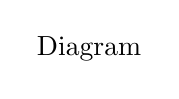
\begin{tikzpicture}
            \node {Diagram};
        \end{tikzpicture}
        \end{center}
    \item A charge \( q \) is surrounded by a closed surface consisting of an inverted cone of height \( h \) and base radius \( R \), and a hemisphere of radius \( R \) as shown in the figure. The electric flux through the conical surface is \( \frac{nq}{6\epsilon_0} \) (in SI units). The value of \( n \) is \underline{\quad} .
    \begin{center}
        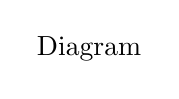
\begin{tikzpicture}
            \node {Diagram};
        \end{tikzpicture}
    \end{center}

    \item On a frictionless horizontal plane, a bob of mass \( m = 0.1 \text{kg} \) is attached to a spring with natural length \( l_0 = 0.1 \text{m} \). The spring constant is \( k_1 = 0.009 \text{Nm}^{-1} \) when the length of the spring \( l > l_0 \) and is \( k_2 = 0.016 \text{Nm}^{-1} \) when \( l < l_0 \). Initially the bob is released from \( l = 0.15 \text{m} \). Assume that Hooke's law remains valid throughout the motion. If the time period of the full oscillation is \( T = (n \pi) \text{s} \), then the integer closest to \( n \) is \underline{\hspace{1cm}}.

    \item An object and a concave mirror of focal length \( f = 10 \text{cm} \) both move along the principal axis of the mirror with constant speeds. The object moves with speed \( v_o = 15 \text{cm s}^{-1} \) towards the mirror with respect to a laboratory frame. The distance between the object and the mirror at a given moment is denoted by \( u \). When \( u = 30 \text{cm} \), the speed of the mirror \( v_m \) such that the image is instantaneously at rest with respect to the laboratory frame, and the object forms a real image. The magnitude of \( v_m \) is \underline{\hspace{1cm}} \( \text{cm s}^{-1} \).

    \begin{center}
        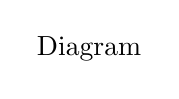
\begin{tikzpicture}
            \node {Diagram};
        \end{tikzpicture}
    \end{center}

    \begin{solution}
        \begin{align*}
            \frac{1}{v} + \frac{1}{u} &= \frac{1}{f} \\
            \intertext{Differentiating with respect to time,}
            \frac{dv}{dt} \left( -\frac{1}{v^2} \right) + \frac{du}{dt} \left( -\frac{1}{u^2} \right) &= 0 \\
            \frac{dv}{dt} &= -\frac{v^2}{u^2} \frac{du}{dt} \\
            \intertext{As, $u$ and $v$ are object distance and image distance with respect to mirror,}
            v_{\textit{image w.r.t. mirror}} &= -\frac{v^2}{u^2} v_{\textit{object w.r.t. mirror}} \tag{1}\\
            \intertext{Now, we can calculate image distance with respect to mirror,}
            \frac{1}{v} + \frac{1}{u} &= \frac{1}{f} \\
            \frac{1}{v} - \frac{1}{30} &= -\frac{1}{10} \\
            \Rightarrow v &= -15 \text{ cm} \tag{2}\\
            \intertext{From equations (1) and (2),}
            v_i - v_m &= -\frac{v^2}{u^2} (v_o - v_m) \\
            0 - v_m &= -\left(\frac{-15}{-30}\right)^2 \left(15-v_m\right)\\
            v_m &= \frac{1}{4}\left(15-v_m\right)\\
            5v_m &= 15\\
            \Rightarrow v_m &= 3 
            \intertext{As every quantity is in cm,}
            \intertext{Therefore, the magnitude of \( v_m \) is \( 3 \text{ cm s}^{-1} \).}
        \end{align*}

    \end{solution}

    \item In the figure, the inner (shaded) region A represents a sphere of radius $r_A = 1$, within which the electrostatic charge density varies with the radial distance $r$ from the center as $p_A = kr$, where $k$ is positive. In the spherical shell B of outer radius $r_B$, the electrostatic charge density varies as $p_B = \frac{2k}{r}$. Assume that dimensions are taken care of. All physical quantities are in their SI units.
    \begin{center}
        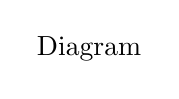
\begin{tikzpicture}
        \node {Diagram};
        \end{tikzpicture}
        \end{center}
    Which of the following statement(s) is(are) correct?
        \begin{tasks}(1)
            \task If $r_B = \sqrt{3}r_A$, then the electric field is zero everywhere outside B.
            \task If $r_B = \frac{3}{2}r_A$, then the electric potential just outside B is $\frac{k}{\varepsilon_0}$.
            \task If $r_B = 2r_A$, then the total charge of the configuration is $15\pi k$.
            \task If $r_B = \frac{5}{2}r_A$, then the magnitude of the electric field just outside B is $\frac{13\pi k}{\varepsilon_0}$.
        \end{tasks}

    \item In Circuit-1 and Circuit-2 shown in the figures, \( R_1 = 1 \Omega \), \( R_2 = 2 \Omega \) and \( R_3 = 3 \Omega \). \( P_1 \) and \( P_2 \) are the power dissipations in Circuit-1 and Circuit-2 when the switches \( S_1 \) and \( S_2 \) are in open conditions, respectively. \( Q_1 \) and \( Q_2 \) are the power dissipations in Circuit-1 and Circuit-2 when the switches \( S_1 \) and \( S_2 \) are in closed conditions, respectively.
    \begin{center}
    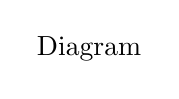
\begin{tikzpicture}
    \node {Diagram};
    \end{tikzpicture}
    \end{center}
    Which of the following statement(s) is(are) correct?
    \begin{tasks}(1)
        \task When a voltage source of \(6V\) is connected across \(A\) and \(B\) in both circuits, \(P_1 < P_2\).
        \task When a constant current source of \(2 Amp\) is connected across \(A\) and \(B\) in both circuits, \(P_1 > P_2\).
        \task When a voltage source of \(6V\) is connected across \(A\) and \(B\) in Circuit-1, \(Q_1 > P_1\).
        \task When a constant current source of \(2 Amp\) is connected across \(A\) and \(B\) in both circuits, \(Q_2 < Q_1\).
    \end{tasks}

    \item A bubble has surface tension \(S\). The ideal gas inside the bubble has ratio of specific heats \( \gamma = \frac{5}{3} \). The bubble is exposed to the atmosphere and it always retains its spherical shape. When the atmospheric pressure is \(P_{a1}\), the radius of the bubble is found to be \(r_1\), and the temperature of the enclosed gas is \(T_1\). When the atmospheric pressure is \(P_{a2}\), the radius of the bubble and the temperature of the enclosed gas are \(r_2\) and \(T_2\), respectively.
    Which of the following statement(s) is(are) correct?
    \begin{tasks}(1)
        \task If the surface of the bubble is a perfect heat insulator, then \( \left(\frac{r_2}{r_1}\right)^5 = \frac{P_{a2} + \frac{2S}{r_2}}{P_{a1} + \frac{2S}{r_1}} \).
        \task If the surface of the bubble is a perfect heat insulator, then the total internal energy of the bubble including its surface energy does not change with the external atmospheric pressure.
        \task If the surface of the bubble is a perfect heat conductor and the change in atmospheric temperature is negligible, then \( \left(\frac{r_2}{r_1}\right)^3 = \frac{2P_{a2}r_2 + \frac{4S}{3}}{2P_{a1}r_1+\frac{4S}{3}} \).
        \task If the surface of the bubble is a perfect heat insulator, then \( \left(\frac{7}{5}r_2\right)^5 = \frac{P_{a2} + \frac{4S}{r_1}}{P_{a1} + \frac{4S}{r_1}} \).
    \end{tasks}

    \item A disk of radius \( R \) with uniform positive charge density \( \sigma \) is placed on the \( xy \) plane with its center at the origin. The Coulomb potential along the \( z \)-axis is \( V(z) = \frac{\sigma}{2\epsilon_0}(\sqrt{R^2 + z^2} - z) \). A particle of positive charge \( q \) is placed initially at rest at a point on the \( z \) axis with \( z = z_0 \) and \( z_0 > 0 \). In addition to the Coulomb force, the particle experiences a vertical force \( F = -c \sqrt{z} \) with \( c > 0 \). Let \( \beta = \frac{2c\sqrt{z_0}}{q\sigma} \). Which of the following statement(s) is(are) correct?
        \begin{tasks}(1)
            \task For \( \beta = \frac{1}{4} \) and \( z_0 = \frac{25}{7} R \), the particle reaches the origin.
            \task For \( \beta = \frac{1}{4} \) and \( z_0 = \frac{3}{2} R \), the particle reaches the origin.
            \task For \( \beta = \frac{4}{3} \) and \( z_0 = \frac{\sqrt{3}}{3} R \), the particle returns back to \( z = z_0 \).
            \task For \( \beta > 1 \) and \( z_0 > 0 \), the particle always reaches the origin.
        \end{tasks}
    \item A double slit setup is shown in the figure. One of the slits is in medium 2 of refractive index \( n_2 \). The other slit is at the interface of this medium with another medium 1 of refractive index \( n_1 (n_2 > n_1) \). The line joining the slits is perpendicular to the interface and the distance between the slits is \( d \). The slit widths are much smaller than \( d \). A monochromatic parallel beam of light is incident on the slits from medium 1. A detector is placed in medium 2 at a large distance from the slits, and at an angle \( \theta \) from the line joining them, so that \( \theta \) equals the angle of refraction of the beam. Consider two approximately parallel rays from the slits received by the detector.
        
        \begin{center}
            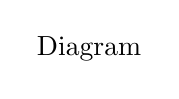
\begin{tikzpicture}
                \node {Diagram};
            \end{tikzpicture}
        \end{center}

        Which of the following statement(s) is(are) correct?
        \begin{tasks}(1)
            \task The phase difference between the two rays is independent of \( d \).
            \task The two rays interfere constructively at the detector.
            \task The phase difference between the two rays depends on \( n_1 \) but is independent of \( n_2 \).
            \task The phase difference between the two rays vanishes only for certain values of \( d \) and the angle of incidence of the beam, with \( \theta \) being the corresponding angle of refraction.
        \end{tasks}

    \item In the given \(P\)-\(V\) diagram, a monoatomic gas \( \left( \gamma = \frac{5}{3} \right) \) is first compressed adiabatically from state \(A\) to state \(B\). Then it expands isothermally from state \(B\) to state \(C\). Given: \( \left(\frac{V_C}{V_B}\right)^{0.6} = 0.5 \), \( \ln 2 = 0.7 \). 
    \begin{center}
        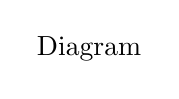
\begin{tikzpicture}
        \node {Diagram};
        \end{tikzpicture}
        \end{center}Which of the following statement(s) is(are) correct?
        \begin{tasks}(1)
            \task The magnitude of the total work done in the process \( A \rightarrow B \rightarrow C \) is \( 144 kJ \).
            \task The magnitude of the work done in the process \( B \rightarrow C \) is \( 84 kJ \).
            \task The magnitude of the work done in the process \( A \rightarrow B \) is \( 60 kJ \).
            \task The magnitude of the work done in the process \( C \rightarrow A \) is zero.
        \end{tasks}

    \item A flat surface of a thin uniform disk of radius R is glued to a horizontal table. Another thin uniform disk B of mass M and with the same radius R rolls without slipping on the circumference of A, as shown in the figure. A flat surface of B also lies on the plane of the table. The center of mass of B has fixed angular speed \(\omega\) about the vertical axis passing through the center of A. The angular momentum of B is \(m\omega R^2\) with respect to the center of A. Which of the following is the value of n?
        \begin{center}
            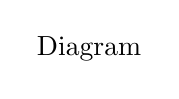
\begin{tikzpicture}
                \node {Diagram};
            \end{tikzpicture}
        \end{center}
        \begin{tasks}(2)
        	\task \(2\)
        	\task \(5\)
        	\task \(\frac{7}{2}\)
        	\task \(\frac{9}{2}\)
        \end{tasks}
    \item When light of a given wavelength is incident on a metallic surface, the minimum potential needed to stop the emitted photoelectrons is \(6.0 \, \text{V}\). This potential drops to \(0.6 \, \text{V}\) if another source with wavelength four times that of the first one and intensity half of the first one is used. What are the wavelength of the first source and the work function of the metal, respectively? [Take \(\frac{hc}{e} = 1.24 \times 10^{-6} \, \text{m} \, \text{V}\)]
        \begin{tasks}(2)
        	\task \(1.72 \times 10^7 \, \text{m}, 1.20 \, \text{eV}\)
        	\task \(1.72 \times 10^7 \, \text{m}, 5.60 \, \text{eV}\)
        	\task \(3.78 \times 10^7 \, \text{m}, 5.60 \, \text{eV}\)
        	\task \(3.78 \times 10^7 \, \text{m}, 1.20 \, \text{eV}\)
        \end{tasks}

    \item Area of the cross-section of a wire is measured using a screw gauge. The pitch of the main scale is 0.5 mm. The circular scale has 100 divisions and for one full rotation of the circular scale, the main scale shifts by two divisions. The measured readings are listed below.
    
    \begin{center}
    \begin{tabular}{|c|c|c|}
    \hline
    Measurement condition & Main scale reading & Circular scale reading \\
    \hline
    Two arms of gauge touching & 0 division & 4 divisions \\
    each other without wire & & \\
    \hline
    Attempt-1: With wire & 4 divisions & 20 divisions \\
    \hline
    Attempt-2: With wire & 4 divisions & 16 divisions \\
    \hline
    \end{tabular}
    \end{center}
    
    What are the diameter and cross-sectional area of the wire measured using the screw gauge?
    
    \begin{tasks}(2)
        \task \(2.22 \pm 0.02 \, \text{mm}, \pi(1.23 \pm 0.02)\text{mm}^2\)
        \task \(2.22 \pm 0.01 \, \text{mm}, \pi(1.23 \pm 0.01)\text{mm}^2\)
        \task \(2.14 \pm 0.02 \, \text{mm}, \pi(1.14 \pm 0.02)\text{mm}^2\)
        \task \(2.14 \pm 0.01 \, \text{mm}, \pi(1.14 \pm 0.01)\text{mm}^2\)
    \end{tasks}
    \item Which one of the following options represents the magnetic field \(\mathbf{B}\) at O due to the current flowing in the given wire segments lying on the xy plane?
    
    \begin{center}
    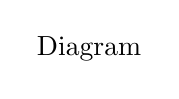
\begin{tikzpicture}
        \node {Diagram};
    \end{tikzpicture}
    \end{center}
    
    \begin{tasks}(2)
        \task \(\mathbf{B} = -\frac{\mu_0 I}{4\pi L}\left(3 + \frac{4}{\pi}\right)\mathbf{k}\)
        \task \(\mathbf{B} = -\frac{\mu_0 I}{4\pi L}\left(\frac{3}{2} + \frac{1}{2\pi}\right)\mathbf{k}\)
        \task \(\mathbf{B} = \frac{\mu_0 I}{4\pi L}\left(\frac{3}{4} + \frac{1}{2\pi}\right)\mathbf{k}\)
        \task \(\mathbf{B} = \frac{\mu_0 I}{4\pi L}\left(\frac{1}{1+4\pi}\right)\mathbf{k}\)
    \end{tasks}
\end{enumerate}






\end{document}
